%!TEX root = ./slopecd.tex
\section{Introduction}\label{sec:introduction}
%%%%%%%%%%%%%%%%%%%%%%%%%%%%%%%%%%%%%%%%%%%%%%

In this paper we present a novel numerical algorithm for Sorted L-One Penalized
Estimation (SLOPE)~\cite{bogdan2013,bogdan2015,zeng2014ordered}, defined as
\begin{problem}\label{pb:slope}
  \min_{\beta \in \mathbb{R}^p}
  P(\beta) = \ell(\beta) + J(\beta)
\end{problem}
% \mm{TODO change}
where we take \(\ell\) to be smooth and twice differentiable and
% \mm{to discuss: $L(X\beta)$ doable? + some computation are sepcific to  the quadratic case}
\begin{equation}
  \label{eq:sorted-l1-norm}
  J(\beta) = \sum_{j=1}^p \lambda_j|\beta_{(j)}|
\end{equation}
is the \emph{sorted \(\ell_1\) norm}, defined through
\begin{equation*}
  |\beta_{(1)}| \geq |\beta_{(2)}| \geq \cdots \geq |\beta_{(p)}| \enspace,
\end{equation*}
with \(\lambda\) being a fixed non-increasing and non-negative sequence.

The sorted $\ell_1$ norm is a sparsity-enforcing penalty that has become
increasingly popular due to several appealing properties, such as its ability
to control false discovery rate~\cite{bogdan2015,kos2020}, cluster
coefficients~\cite{figueiredo2016, schneider2020a}, and recover sparsity and
ordering patterns in the solution~\cite{bogdan2022}. Unlike other competing
sparse regularization methods such as MCP~\cite{zhang2010} and
SCAD~\cite{fan2001}, SLOPE is also a convex problem~\cite{bogdan2015}.

In spite of the availability of predictor screening
rules~\cite{larsson2020c,elvira2022}, which help speed up SLOPE in the
high-dimensional regime, current state-of-the-art algorithms for SLOPE perform
poorly in comparison to those of more established penalization methods such as
the lasso (\(\ell_1\)-norm regularization) and ridge regression
(\(\ell_2\)-norm regularization). As a small illustration of this issue, we
compared the speed at which the SLOPE and glmnet packages fit a complete
regularization path for the bcTCGA data set. SLOPE takes x seconds to fit the
full path, whilst glmnet requires only y seconds. \mm{put result here and
details in experiment section}

This lackluster performance has hampered the applicability of SLOPE to many
real-world applications. A major reason for why algorithms for solving
$\ell_1$-, MCP-, or SCAD-regularized problems enjoy better performance is that
they use coordinate
descent~\cite{tseng2001convergence,friedman2010,breheny2011}. Current SLOPE
solvers, on the other hand, rely on proximal gradient descent algorithms such
as FISTA~\cite{beck2009} and the alternating direction method of multipliers
method (ADMM)~\cite{boyd2010}, which have proven to be less inefficient than
coordinate descent in empirical benchmarks on related problems, such as the
lasso~\cite{moreau2022benchopt}. Applying coordinate descent to SLOPE is not,
however, straightforward since convergence guarantees for coordinate descent
require the objective to be separable, which is not the case for SLOPE. As a
result, naive coordinate descent schemes can get
stuck~(\cref{fig:naive-cd-stuck}).

\begin{figure}[htpb]
  \centering
  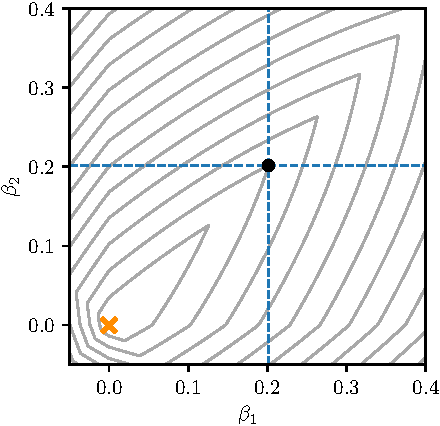
\includegraphics[]{naive-cd-stuck.pdf}
  \caption{%
    An example of (standard) coordinate descent getting stuck on a two-dimensional SLOPE problem.
    The main plot shows level curves for the primal objective~\eqref{pb:slope}, with the optimum \(\beta^* = [0, 0]^T\) indicated by the orange cross.
    The marginal plots displays objective values at \(\beta_1 = 0.2\) when optimizing over \(\beta_2\) and vice versa.
    At \(\beta = [0.2,0.2]^T\), a naive coordinate descent algorithm can only move in the directions indicated by the dashed lines---neither of which are descent directions for the objective.
    As a result, the algorithm is stuck.
  }
  \label{fig:naive-cd-stuck}
\end{figure}

% The resulting solution \(\hat{\beta}\) has the property that it can cluster the
% coefficients by their magnitudes, such that \(\mathcal{C}=
% \{j: |\beta_j|=c\}\) for some \(c\).

In this article we address this problem by introducing a new, highly effective
algorithm for SLOPE based on a hybrid proximal gradient and coordinate descent
scheme. Our method features convergence guarantees and reduces the time
required to fit SLOPE by orders of magnitude in our empirical experiments.
